\documentclass[twocolumn, 11pt]{article}%
\usepackage{amsmath, amssymb, esint, gensymb, hyperref, mathtools}
\usepackage{graphicx, cuted, geometry, float, scalerel, xcolor, xfrac}

\newcommand\sbullet[1][.5]{\mathbin{\ThisStyle{\vcenter{\hbox{%
  \scalebox{#1}{$\SavedStyle\bullet$}}}}}%
}

\geometry{
    a4paper,
    total={170mm,260mm},
}

\begin{document}

\begin{strip}
  \vspace*{\dimexpr-\stripsep}
  \begin{center}
      \Large\textbf{FISIKA 2}\\
      \large{Pertemuan 1 - Minggu 6 (302170)}\\
      \large{\today}
   \end{center}
\end{strip}

\section{Arus Listrik Dan Kerapatan Arus}
    \paragraph{} Arus listrik didefinisikan sebagai jumlah muatan positif yang lewat penampang dalam satuan waktu.
    \[ I=\frac{dQ}{dt} \]
    Satuan arus adalah coulomb per detik atau disebut ampere.
    \[ 1\ \sfrac{C}{s} = 1 A \]
    Suatu konduktor dengan luas penampang A. Bila dalam selang waktu dt telah lewat muatan positif sebesar dQ, maka dQ adalah besar muatan total yang terdapat di dalam tabung volume (A.v.dt), dengan v adalah kecepatan rata-rata partikel pembawa muatan. Bila jumlah partikel satuan volume n, dan muatan tiap-tiap partikel q, maka:
    \[ dQ=A.vdt.n.q \]
    Sehingga kuat arus I adalah
    \[ I=\frac{dQ}{dt}=A.v.n.q \]
    Rapat arus (J) didefinisikan sebagai kuat arus I dibagi luas penampang
    \[J=\frac{I}A\]

    \section{Konduktivitas dan Resistivitas}%
    \paragraph{} Konduktivitas listrik didefinisikan sebagai perbandingan antara rapat J dengan kuat medan listrik E yang menimbulkan arus. Dengan kata lain konduktivitas adalah kemampuan mengalirkan arus listrik dari sebuah zat.
    \[\sigma = \frac{J}E \]

    dengan
    \[ E=-\frac{dV}{dx} \]
    \begin{align*}
    J&=\frac{I}A =\sigma E\\
    J&=\frac{I}A =\sigma \left(-\frac{dV}{dx}\right)\\
    \end{align*}

    atau
    \begin{align*}
        I&= \sigma A \left(-\frac{dV}{dx}\right)\\
        I\ dx&= -\sigma A dV\\
        I\int\limits_0^L dx &= -\sigma A \int\limits_a^b dV\\
        IL&=-\sigma A(V_b -V_a)\\
        IL&= \sigma AV_{ab}\\
        V_{ab} &= \frac{IL}{\sigma A}
    \end{align*}

    Konstanta $\displaystyle \frac{L}{\sigma A}$ disebut \textbf{tahanan listrik (hambatan listrik)} dari kawat dan diberi notasi \textbf{R}, jadi

    \[R=\frac{L}{\sigma A}\]
    \[V_{ab}=IR \]

    Jika arus I dalam ampere, beda potensial V dalam volt, maka tahanan R dalam ohm ($\Omega$), maka satuan $\sigma$ adalah

    \[\frac1{ohm.m} \]

    Kebalikan dari kondukivitas didefinisikan sebagai resistivitas $\rho$, sehingga
    \[\rho=\frac1{\sigma} \]

    Satuan kondukivitas adalah ohm.m ($\Omega.m$)\\

    Sehingga hambatan listrik dari kawat dengan Panjang L, luas penampang A, dan resistivitas $\rho$ adalah

    \[ R=\rho\frac{L}A \]

    \section{Daya Listrik}%
    Secara definisi daya adalah usaha per satuan waktu, atau energi per satuan waktu.

    \begin{align*}
        dW&=dQ(V_a-V_b)\\
        dW&= I\ dt\ V_{ab}\\
        P&=\frac{dW}{dt}=IV_{ab}
    \end{align*}
    Jika terdapat suatu hambatan \textbf{R}, maka

    \begin{align*}
        P&=I^2R\\
        P&= \frac{V^2_{ab}}{R}
    \end{align*}

    \section{Rangkaian Arus Searah}%
    \begin{center}
        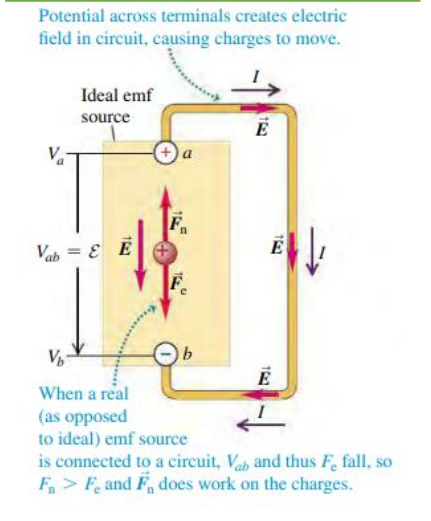
\includegraphics[width=200px]{2.png}
    \end{center}
    Untuk sumber tegangan ideal dan dihubungkan dengan hambatan luar \textbf{R}, adalah
    \[ \epsilon = V_{ab} =IR\]
    \begin{center}
        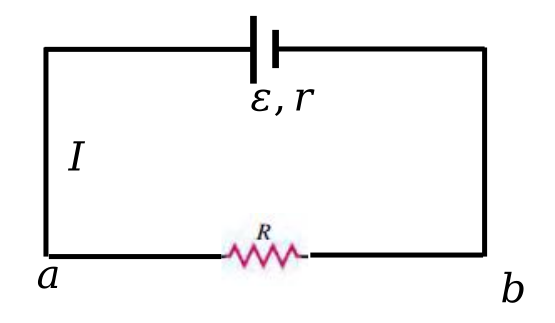
\includegraphics[width=100px]{1.png}
    \end{center}
    \begin{align*}
        V_{ab}&=IR\\
        &=\epsilon-Ir\\
        I&=\frac{\epsilon}{r+R}
    \end{align*}

    Lambang $\epsilon$ disini adalah GGL (Gaya Gerak Listrik) atau dalam bahasa Inggri disebut Electromotive Force. $\epsilon$ ini adalah tegangan listrik sumber sebelum dihubungkan dengan rangkaian tertutup, lalu V adalah tegangan setelah disambungkan dalam rangkaian tertutup. Tegangan baterai dalam rangkaian pasti lebih sedikit daripada GGL nya, karena setiap baterai mempunyai hambatan dalam.

    \section{Rangkaian Hambatan}%
    \subsection{Rangkaian Seri}%
    Dalam rangkaian seri, resistansi dari seluruh rangkaian ditambahkan. Sedangkan arus yang mengalir di sepanjang rangkaiannya adalah sama.
    \[R = R_1 +R_2+R_3+R_4 \]
    \[V_{ab} = I\times R_1 + I\times R_2 + I\times R_2 \]
    \[I\times R_{ab} = I\times R_1 + I\times R_2 + I\times R_2 \]

    \subsection{Rangkaian Paralel}%
    Dalam rangkaian paralel
    \[I=I_1 + I_2 + I_3 \]
    \[\frac{V_{ab}}{R_{ab}} = \frac{V_{ab}}{R_1}+\frac{V_{ab}}{R_2}+\frac{V_{ab}}{R_3} \]
    \[\frac{1}{R_{ab}} = \frac{1}{R_1}+\frac{1}{R_2}+\frac{1}{R_3} \]
\end{document}
